\documentclass[11pt, a4paper]{article}
\usepackage[utf8]{inputenc} % comment when using lualatex
\usepackage{fullpage}
\usepackage{graphicx}
\usepackage[hidelinks]{hyperref,xcolor}
\renewcommand\UrlFont{\color{blue}\rmfamily}

% Bibliography management
%  see https://www.overleaf.com/learn/latex/Biblatex_citation_styles
%  and https://www.overleaf.com/learn/latex/Bibliography_management_in_LaTeX
% to use overleaf with reference manager
%  see: https://no.overleaf.com/blog/639-tip-of-the-week-overleaf-and-reference-managers
\usepackage[backend=biber]{biblatex}
\addbibresource{library.bib} %Imports bibliography file
 
% Title of your study
\title{Study Title}

% Your name(s)
\author{Jane \textsc{Doe}}

% Your supervior(s)
\newcommand{\supervisors}{Oli \textsc{Nordmann}
\\Kari \textsc{Nordmann}}

% Time period for the study
%    Autumn project?, Master's thesis?, Autumn and master?, Other? What?
\newcommand{\timePeriod}{Autumn project and Master's thesis}

% Amount of resources in PM planned
% E.g. 20 hours x week for autumn project 
% + 40 hours x week for the master thesis (a semester is normally 14 weeks)
\newcommand{\resourcesPlanned}{1680 hours (20h per week during autumn, 40h per week during master)}

 % Web address for the project (if any)
\newcommand{\homepage}{\url{https://www.ntnu.edu/idi/}}

% Date for title page, default is today
\date{\today}

\makeatletter{}

\begin{document}

% Your research plan follows in the next page. Your final deliverable should be:
%     • A maximum of four pages, including this front page.
%     • The three pages following this front page should include everything: figures, tables, references.
%     • The total word count should not exceed 1200 words. So do not try to reduce the size of the font or line spacing to get more text into those three pages.
%     • When you are finished and before you deliver, you can delete all the help text, which is gray and is in cursive like this text. 

% Title page based on https://www.latextemplates.com/template/academic-title-page
\begin{titlepage}
  	\newcommand{\HRule}{\rule{\linewidth}{0.3mm}} % Defines a new command for horizontal lines, change thickness here
	\center % Centre everything on the page
	%------------------------------------------------
	%	Headings
	%------------------------------------------------
	
	\textsc{\LARGE Norwegian University of Science and Technology}\\[1.5cm]
	
	\textsc{\Large Plan for Research Studies}\\[0.5cm]
	
	\textsc{\large TDT 39 - Empirical studies in IT}\\[0.5cm]
	
	%------------------------------------------------
	%	Title
	%------------------------------------------------
	
	\HRule\\[0.4cm]
	
	{\huge\bfseries \@title}\\[0.4cm]
	
	\HRule\\[1.5cm]
	
	%------------------------------------------------
	%	Author(s)
	%------------------------------------------------
	\begin{minipage}{0.4\textwidth}
		\begin{flushleft}
			\large
			\textit{Author(s)}\\
			\@author % Your name
		\end{flushleft}
	\end{minipage}
	~
	\begin{minipage}{0.4\textwidth}
		\begin{flushright}
			\large
			\textit{Supervisor(s)}\\
			\supervisors % Supervisor's name
		\end{flushright}
	\end{minipage}
	
% 	If you don't want a supervisor, uncomment the two lines below and comment the code above
% 	{\large\textit{Author(s)}}\\
% 	\@author % Your name
	
	%------------------------------------------------
	%	Date
	%------------------------------------------------
	
	\vfill\vfill
		{\large\today} % Date, change the \today to a set date if you want to be precise
    \vfill\vfill
	
    
    \footnotesize{Time period: \timePeriod}
    \\[0.3cm]
    \footnotesize{Resources planned: \resourcesPlanned}
    \vfill
    \homepage
    
    \vfill
    
    %------------------------------------------------
    % Change log for the plan (can be deleted before delivery)
    % When you update the plan please record what you changed and what the reason for the change. This will be useful for your supervisor.
    %------------------------------------------------
    \begin{tabular}{ | l | l | l | l |}
    \hline
    \textbf{Version} & \textbf{Date of change} & \textbf{What is changed?} & \textbf{The reason for the change} \\ \hline
    0.1 & 03-10-2010 & first version & \\
    \hline
\end{tabular}
	
	%------------------------------------------------
	%	Logo
	%------------------------------------------------
	\vfill\vfill
	
\includegraphics[width=0.3\textwidth]{./hovedlogo_eng.png}
	\vfill
	 
	\vfill
	
\end{titlepage}


% This plan is based on the 6Ps of research as described in Oates, Dr Briony J (2005). Researching Information Systems and Computing. SAGE Publications, enhanced based on Creswell, J. W. (2014). Research design- Qualitative, quantitative, and mixed methods approaches (4th ed.). SAGE Publications. Version of September 2019.

\section*{Purpose}
% "Describe the reason for doing the research, the topic of interest, why it is important or useful to study this, the specific research question(s) asked and the objectives set. Research without a purpose is unlikely to be good research." (Oates 2005)
% Write in this section about the following:
%     • What is the problem? Whose problem is it? Refer to 2-3 good scientific references that confirm for the reader that this is actually a relevant problem.
%     • What is done earlier to address this problem? Give 4-5 good references that illustrate the different approaches taken by other researchers to solve this problem. (you might also consider to do an in-depth literature review as part of your autumn project).
%     • What is wrong with earlier research? Did they not manage to solve the problem? Why? Why is your approach going to be better? What new knowledge do you plan to add?
%     • Summarize with a list of clearly defined research questions. One main question and 2-3 sub-questions related to the main question. Note that the sub-questions should contribute to answer the main question.

Write your own text here

\section*{Contributions}
% "Describe the outcomes of research, especially your contribution to knowledge about your subject area. Your contribution can be an answer to your original research question( s) but can also include unexpected findings. For example, you and the academic community might learn something about a particular research strategy as a result of your research. Your thesis, dissertation, conference paper or journal article is also a product of your research. For those research projects that involve design and creation, a new computer-based product or new development method could also be a product of your research." (Oates 2005)
% Types of research products: 1) new or improved evidence; 2) new or improved methodology; 3) new or improved analysis; 4) new or improved concepts or theories; 5) new or improved computer-based product.
% Write in this section about the following:
%     • What will be your research contribution? Which of the four types above?
%     • How and why will it be better than earlier contributions?

Write your own text here

\section*{Research Method}
% "Describe the sequence of activities undertaken in any research project. The process involves identifying one or more research topics, establishing a conceptual framework (the way you choose to think about your research topic), the selection and use of a research strategy and data generation methods, the analysis of data and the drawing of conclusions, including recognizing any limitations in your own research. As explained already, the process should be carried out systematically if the research is to be accepted as rigorous."
% Write here your (See the figure below from Oates 2005):
%     • Research strategy (survey, case study, action research, experiment, design etc.)
%     • Is this mixed-method? Then you can have different strategies for different steps in the design.
%     • Data generation methods (interview, focus group, observation, documents etc.)
%     • You can have more than one data generation method for each strategy.
%     • Data analysis methods (qualitative or quantitative.)

Write your own text here

\section*{Participants}
% "These include those whom you directly involve in your research, for example by interviewing them or observing them, and also those who are indirectly involved, such as the editors to whom you submit a research paper. It is important that you deal with all these people legally and ethically, that is, you do not do anything that might annoy them or cause them harm (physically, mentally or socially). You yourself as a researcher are also a research participant. As we shall see later, for some types of research, researchers are expected to be objective and remain largely unseen in the reporting of their research, whereas in other types of research the researchers are open about their feelings and how their presence influenced the other participants and the research situation."
% You need to clarify the following:
%     • Who are the informants? How do you plan to recruit them?
%     • If you want to collect data you should take care of the ethical issues. E.g. 1) you should get approval from NSD before you start collecting data, 2) you should have users sign informed consent forms, 3) you should make sure you don't share person-related data (e.g. you cannot have this data on Google doc!).
%     • Don't underestimate use recruitment. It is often the part of the research that shows to be the most problematic! Get started early.
%     • Who are the researchers?
%     • Be specific who will do what in the project.

Write your own text here

\section*{Research Paradigm}
% "A pattern or model or shared way of thinking. Managers sometimes talk of the need for a ‘paradigm shift’ to mean that a new way of thinking is required. In computing, we talk about programming language paradigms, for example, a group of languages that share a set of characteristics, such as the object-oriented paradigm (for example, Smalltalk and C + +). Here we are concerned with the philosophical paradigms of research. Any piece of research will have an underlying paradigm. We have noted already that different academic communities and individuals have different ideas about the kinds of research questions to ask and the process by which to answer them because they have different views about the nature of the world we live in and therefore about how we might investigate it. These different views stem from different philosophical paradigms. We shall look at three such paradigms: ‘positivism’, interpretivism’ and ‘critical research’ – each will be explained later."

Write your own text here

\begin{figure}[h]
    \center
    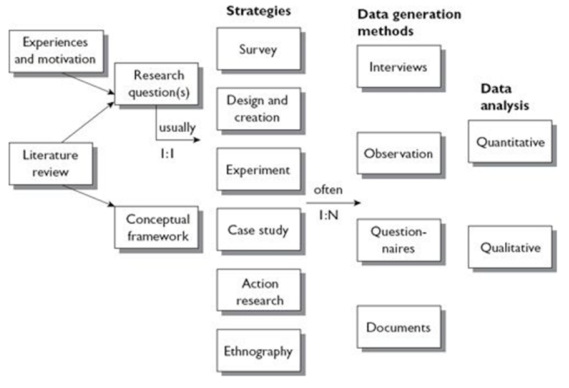
\includegraphics[width=0.5\textwidth]{research-strategies.png}
    \caption{Research strategies \cite{oates2005researching}}
    \label{fig:research_strategies}
\end{figure}

\section*{Final Deliverables and Dissemination}
% "The means by which the research is disseminated and explained to others. For example, it may be written up in a paper or thesis, or a conference paper is presented to an audience of conference delegates, or a computer-based product is demonstrated to clients, users or examiners. It is imphttps://www.overleaf.com/learn/latex/Biblatex_citation_stylesortant that the presentation is carried out professionally – otherwise your audience might assume your whole research project was not undertaken in a professional manner."

Write your own text here

% References
\printbibliography 

\end{document}
